\documentclass{elsarticle}
\usepackage{graphicx}
%\usepackage{multicol}
%\usepackage{footmisc}
\usepackage{amstext}
\usepackage{amsmath}
\usepackage{amssymb}
\usepackage{amsthm}
\usepackage[english]{babel}
%\usepackage[official,right]{eurosym}
\selectlanguage{english}
\hyphenation{ExecEngine}
\newtheorem{lemma}{Lemma}
\begin{document}
% Ampersand -----------------------------------------------------------

%\def\id#1{\text{\it #1\/}}
\newcommand{\id}[1]{\text{\it #1\/}}
\newcommand{\code}[1]{\text{\tt\small #1}}
\newcommand{\stmtText}[1]{``{\small\tt #1}''}
\newcommand{\dom}[1]{\id{dom}(#1)}
\newcommand{\cod}[1]{\id{cod}(#1)}
\renewcommand{\int}[2]{\id{inter}(#1,#2)}
\newcommand{\relsIn}[1]{\id{relsIn}(#1)}    % maps a Term to a set of Relations
\newcommand{\maintain}{\id{maint}}
\newcommand{\pop}[2]{\id{pop}_{#1}(#2)}
\newcommand{\inst}{\id{inst}}
\newcommand{\relname}[1]{\id{relname}(#1)}
\newcommand{\src}[1]{\id{src}(#1)}
\newcommand{\tgt}[1]{\id{tgt}(#1)}
\newcommand{\sat}[2]{\id{sat}_{#1}(#2)}
\newcommand{\viol}[2]{\id{viol}_{#1}(#2)}
\newcommand{\sign}[1]{\id{sign}(#1)}
\newcommand{\powerset}[1]{\cal{P}\{#1\}}
\newcommand{\theCode}{\url{http://cs.ru.nl/~B.Joosten/ampTypes/}}
\newcommand{\la}{\langle}
\newcommand{\ra}{\rangle}
\newcommand{\full}{V}
\newcommand{\declare}[3]{\id{#1}_{\pair{#2}{#3}}}
\newcommand{\subst}[3]{#3_{[#1\rightarrow #2]}}
\newcommand{\fullt}[2]{V_{\pair{#1}{#2}}}
\newcommand{\iden}{I}
\newcommand{\ident}[1]{I_{\id{#1}}}
\newcommand{\expr}[3]{(#1)_{#2\times #3}}
\newcommand{\pair}[2]{\la{#1},{#2}\ra}
\newcommand{\Pair}[2]{#1\times#2}
\newcommand{\pairs}[1]{\id{pairs}(#1)}
\newcommand{\triple}[3]{\la{#1},{#2},{#3}\ra}
\newcommand{\quadruple}[4]{\la{#1},{#2},{#3},{#4}\ra}
\newcommand{\atom}[1]{{\tt\small #1}}
\newcommand{\atoms}{\mathcal{A}}
\newcommand{\Atoms}{\mathbb{A}}
\newcommand{\concept}[1]{{\tt\small #1}}
\newcommand{\concepts}{\mathcal{C}}
\newcommand{\Concepts}{\mathbb{C}}
\newcommand{\decls}{\mathcal{D}}  %% names of relations
\newcommand{\rels}{\mathcal{R}}   %% all relations
\newcommand{\Rels}{\mathbb{R}}   %% all relations
\newcommand{\relations}{\mathcal{M}} % representing terms. M is a subset of R.
\newcommand{\triples}{\mathcal{T}}
\newcommand{\Triples}{\mathbb{T}}
\newcommand{\Triple}[3]{#1\times#2\times#3}
\newcommand{\vertices}{N}
\newcommand{\rules}{\mathcal{U}}
\newcommand{\Rules}{\mathbb{U}}
\newcommand{\specrules}{\mathcal{S}}
\newcommand{\roles}{\mathcal{O}}
\newcommand{\Events}{{\mathit E}}
\newcommand{\dataset}{\mathscr{D}}
\newcommand{\Dataset}{\mathbb{D}}
\newcommand{\schema}{\mathscr{Z}}
\newcommand{\functionality}{\mathscr{F}}
\newcommand{\select}[2]{\id{select}_{#1}\{{#2}\}}
\newcommand{\migrsys}{\mathscr{M}}
\newcommand{\infsys}{\mathscr{S}}
\newcommand{\tf}[1]{\mathscr{T}(#1)}
\newcommand{\ptf}[1]{\mathscr{T}'(#1)}
\newcommand{\ti}[1]{\mathscr{I}(#1)}
\newcommand{\tic}[1]{I_{\cal C}(#1)}
\newcommand{\relAdd}{\dagger}
\newcommand{\flip}[1]{{#1}^\smallsmile} %formerly:  {#1}^\backsim
\newcommand{\kleeneplus}[1]{{#1}^+}
\newcommand{\kleenestar}[1]{{#1}^*}
\newcommand{\cmpl}[1]{\overline{#1}}
\newcommand{\rel}{\times}
\newcommand{\compose}{;}
\newcommand{\subs}{\subseteq}%{\models}
\newcommand{\fun}{\rightarrow}
\newcommand{\isa}{\preceq}
%\newcommand{\isaClos}{\sqsubseteq}
\newcommand{\typetest}{?}
\newcommand{\meet}{\sqcap}
\newcommand{\join}{\sqcup}
\newcommand{\Meet}{\bigsqcap}
\newcommand{\Moin}{\bigsqcup} % because LaTeX has already defined command \Join.
\newcommand{\order}{\ominus}
\newcommand{\anything}{\top}
\newcommand{\nothing}{\bot}
\newcommand{\rewriteto}{\rightarrow}
\newcommand{\calc}{\implies}
\newcommand{\alland}{\bigwedge}
\newcommand{\mph}[3]{#1_{#2\times #3}}
\newcommand{\mphu}[1]{#1_{\univ\times\univ}}

%-----------------------------------------
\newcommand{\kse}{\hspace*{1.7em}}
\newcommand{\ksf}{\hspace*{1em}}
\newcommand{\ksg}{\hspace*{1em}}
\newenvironment{derivation}{\begin{tabbing}\kse \= \ksf \= \ksg \= \kill}{\end{tabbing}}
\newtheorem{definition}{Definition}
\newcommand{\term}[1]{\>\>\(#1\)\\[1ex]}
\newcommand{\rela}[2]{\>\(#1\)\>\>\{ \ #2 \ \}\\[1ex]}
\newcommand{\weg}[1]{}

\def\define#1{\label{dfn:#1}{\em #1}\index{#1}}
\def\definem#1{\label{dfn:#1}{\em #1}\index{#1}\marge{#1}}
\newcommand{\marg}[1]{\index{#1}\marge{#1}}


% TODO Algemeen:
% - type van triple-set en atom-set definieren zodat viol_u ?->P(?x?)
%   (Bas: ik heb foute types weggehaald, maar dit nog niet gedefinieerd)
% - nieuwe populatie na de disjoint union zou de populatie met ENFORCE regels toegepast moeten zijn
%  (en in het bijzonder de ISA regels)

% TODO Stef:
% - stukje literatuuronderzoek
% https://ieeexplore.ieee.org/abstract/document/7445334?casa_token=ECzi6XeV2ncAAAAA:KhWzB8XBFOUJ0C6AD-XjX_ryuA9ARvTd3gm6RR-ZNiR8sZ1858FJpQ7zKQhkAZDlv8IjPdgD
% https://ieeexplore.ieee.org/abstract/document/8549944?casa_token=9qiGqNzh2Q0AAAAA:C-cYogExB35nGxQdxLcdBh4JoLNvM0OHedAMhCbB5V4kb4_6nzHUvc23xSJbeoBu67LSiz-Y
% https://citeseerx.ist.psu.edu/viewdoc/download?doi=10.1.1.651.9298&rep=rep1&type=pdf
% https://www.scirp.org/html/4-7800724_106592.htm
% https://www.researchgate.net/profile/Ranjana-Badre/publication/318665687_GUI_for_Data_Migration_and_Query_Conversion/links/5b45bbea0f7e9b1c722386e5/GUI-for-Data-Migration-and-Query-Conversion.pdf
% https://journal3.uin-alauddin.ac.id/index.php/literatify/article/view/12567

% Bewijsverplichtingen:
% -> het migratie-systeem is typefout-vrij (opmerking: als we de type-checker buiten beschouwing willen laten, kunnen we dit niet beschrijven)
% -> het migratie-systeem is vrij van overtredingen op regels die het migratie-systeem moet bewaken
% -> het migratie-systeem bevat alle oude data, ihb nog steeds na het toepassen van de enforce regels
% -> er is een pad naar ingebruikname van het nieuwe systeem (vanaf de initiële toestand van het migratie-systeem)
% -> corollary: op het moment van ingebruikname van het nieuwe systeem, is het migratie-systeem vrij van overtredingen op regels die het nieuwe systeem moet bewaken
% -> optioneel: na een begrensd aantal 'voortgangs-stappen' kan het nieuwe systeem in gebruik genomen worden
% -> optioneel: er bestaat een migratie-systeem dat de oude functionaliteit behoudt (mogelijk uitbreid) totdat het nieuwe systeem in gebruik genomen is?

\title{A Theory for Data Migration of Generated Evolving Information Systems}
\author[ou,ordina]{Stef Joosten\fnref{fn1}}
\ead{stef.joosten@ou.nl}
\author[umn]{Sebastiaan Joosten\fnref{fn2}}
\address[ou]{Open Universiteit Nederland, Heerlen, the Netherlands}
\address[ordina]{Ordina NV, Nieuwegein, the Netherlands}
\address[umn]{University of Minnesota, Minneapolis, USA}
\fntext[fn1]{ORCID 0000-0001-8308-0189}
\fntext[fn2]{ORCID 0000-0002-6590-6220}

\begin{abstract}
   The Ampersand project has provided the theory and tools to generate information systems from an algebraic specification.
   However, information systems in practice may change repeatedly after their maiden deployment.
   Changes that affect the data model typically result in a data migration.
   In such cases, simply regenerating the system is not enough.
   That would reset the database to its initial state, losing all data gathered so far.
   To prevent that, a migration engineer must transfer the old data to the new system by hand.

   In this contribution we develop a theory for reliable data migration to help the migration engineer
   to transfer the data and preserve the semantics as much as possible.
   We aim to automate the data migration,
   to prevent mistakes and enable more frequent migrations.
   The target is to generate a migration script from two specifications: the old specification and the new specification.
   A software generator that embodies this theory is subject of future research.
\end{abstract}

\begin{keyword}
relation algebra\sep software development\sep data migration\sep software migration\sep Ampersand
\end{keyword}
\maketitle

\section{Introduction}
\label{sct:Introduction}
   We believe in generating information systems%
\footnote{In the sequel, the word ``system'' refers to the phrase ``information system''. This simplifies the language a little. }
   to prevent human errors.
   By generating rather than programming systems by hand,
   we avoid introducing errors in the translation from design to a concrete system.
   A mistake not made cannot propagate into production.
   For this purpose, we use an existing compiler, Ampersand~\cite{Joosten-JLAMP2018},
   that generates a system from an Ampersand script.
   An Ampersand script contains just enough information to generate a complete system,
   which means that a classical database schema (i.e. data structure plus semantics) can be extracted from the Ampersand script.
   For the purpose of this paper we can equate an Ampersand script with the schema of the generated system.

   We also believe that information systems should be released into production in small increments,
   to obtain shorter release cycles, more frequent releases, and thus a more agile software development process%
   \footnote{These effects can be measured in terms of DevOps metrics such as
   deployment frequency,
   reliability of deployments, and
   change failure rate~\cite{DevOps2021}.}.
   By installing upgrades automatically, frequently and in small increments,
   users experience an evolving system.

   We recognize that designs from which concrete systems are generated can have errors in them:
   Either an engineer was making a mistake directly,
   or the requirements the engineer was taking into account were miscommunicated,
   or the environment changed in a way that was not foreseen.
   Regardless of the reason, even a generated system may need to be repaired.
   For this reason, we focus on evolving systems.
   
   This paper studies this evolution in increments, in which we distinguish an ``old system'' and a ``new system''.
   In each increment we need to migrate the data from the old system to the newly designed system.
   This situation poses specific requirements to data migration.
   For instance, if a data migration has other purposes than just to evolve a system,
   e.g.~\cite{Gholami2016,Bisbal1999},
   migration engineers may want to preserve the functionality to avoid introducing new errors in an otherwise error-prone process.
   When one system evolves into another, however, preserving the functionality is not an option.
   To change the functionality is the very purpose of the evolution.
   So, we must make sure to use methods for data migration that are specifically meant for evolving systems.
   
   Information systems are typically used by distributed actors (both users and computers) who continually work with data.
   A system $\infsys$ contains a dataset $\dataset_{\infsys}$, which represents the state of the system.
   (In the sequel we may just write $\dataset$
   if the corresponding system is either clear from the context or irrelevant for the argument.)
   Every event that an actor causes in system $\infsys$ may change the state $\dataset$ of that system.
   Data migration occurs when an old system, $\infsys$, is replaced by a new system, $\infsys'$,
   while preserving the meaning of the data from $\infsys$ as much as possible.
   Just copying the set of data from $\infsys$ to $\infsys'$ is obviously wrong if the schemas of both systems differ.
   
   The schema $\schema_{\infsys}$ of a system $\infsys$ is basically a set of semantic constraints on its dataset $\dataset$.
   (We will denote the schema just as $\schema$ if the system is obvious or irrelevant to know.)
   The Ampersand compiler generates systems that keep all constraints satisfied at all times.
   Much like~\cite{Spivak2012}, our work assumes that the semantics of the old dataset is encoded in its schema,
   so we can be explicit about ``preserving the meaning as much as possible''.
   In contrast with~\cite{Spivak2012}, our approach does not work with functions (functors)
   but with relations in a way that bears resemblance with Alloy~\cite{Alloy2006} and allegories%
   \footnote{Allegories are a specific type of categories, which the reader does not need to understand for the purpose of this paper}~\cite{Zielinski2013}.

   The theory we develop in this paper must lead to tools that satisfy such practical requirements as
   zero down-time updates and ways to cope with data pollution.
   In practice, more frequent updates require that updates have zero down-time.
   For our theory, zero down-time means that the release of new functionality may not be delayed by anything a migration engineer must do.
   
   Extra complications arise from accumulated data pollution in the old system.
   This allows us to categorize data pollution in the old system in the following categories:
   \begin{itemize}
      \item data pollution that cannot be captured in constraints on the dataset,
      such as a street address that has become obsolete because the person failed to send a change of address.
      \item data pollution that violates a constraint in the schema.
      \item data pollution that violates a constraint that is not in the schema.
      \item data pollution that is a consequence of an erroneous constraint in the schema.
   \end{itemize}
   The first category of pollution must be dealt with by working procedures, to prevent such pollution as much as possible.
   In some cases, constraints on data can be formulated,
   so the system can help the user and simplify (or eliminate) the corresponding working procedure.
   Such constraints move this type of pollution to one of the other categories.
   The second category, violations of constraints from the schema, does not occur in our work.
   Since the old system $\infsys$ was generated by Ampersand,
   $\infsys$ keeps all constraints from the schema satisfied at all times.
   This sets our approach apart from other approaches to formalize data migration, e.g.~\cite{Thalheim2013}.
   Data pollution that is not captured by any of the constraints mentioned in the schema
   can be dealt with by adding constraints in the new system $\infsys'$.
   In that case, a migration engineer must ensure that $\infsys'$ can start with data that satisfies all constraints in its schema.
   So some human intervention may be necessary.
   The last category of data pollution, erroneous constraints, must be fixed by replacing them by the correct constraints in $\infsys'$.

   This illustrates that automating data migrations also has its limits.
   Some effort of a migration engineer may be required.
   If the semantics encoded in the new schema $\schema'$ differs from the old schema $\schema$,
   a migration engineer must make choices on how to interpret existing data in the new schema.
   She may even want to adapt data of which the constraints in the schema have not changed.
   This requires a third schema, $\schema_m$, which specifies the migration itself.
   We generate $\schema_m$ in the form of source code, so the migration engineer can change everything she wants to suit the particulars of the data migration.
   In the sequel, automation of data migration means to generate the schema $\schema_m$.

   The benefits of automating data migrations work in two directions.
   The automation itself saves effort and errors,
   contributing to more frequent and smaller releases.
   Smaller and faster releases also mean smaller migrations
   and therefore a smaller difference between $\infsys$ and $\infsys'$.
   The smaller that difference, the simpler the migration and the more of it can be automated.

   The contribution of this paper is to derive a migration schema $\schema_m$ from an existing system $\infsys$
   (which has its own schema and dataset) and a new schema $\schema'$.
   A formal understanding of data migration will help to automate data migrations correctly and reliably.
   Our theory is based on the following assumptions:
\begin{itemize}
   \item the old data set may be polluted, but it satisfies its schema;
   \item the data migration may require human interaction, which may take time;
   \item the part of the data that does not change can be migrated automatically;
   \item the meaning of data must be preserved, at least for the data that does not change;
   \item the business must continue during the migration without interruption;
   \item the part of the migration that can be automated is usually not sufficient;
         it takes additional human creativity to complete the migration specification;
   \item there is a compiler to generate an information system from a given schema.
         In this work, we use the Ampersand compiler for that purpose.
\end{itemize}

\section{Migration steps}
   A smooth migration would ideally proceed as follows:
   Launch the new system in parallel to the old one, copy data from the old to the new system, and have everyone use the new system.
   However, numerous issues might impede that plan.
   The following examples illustrate the practical issues that may occur:
\begin{enumerate}
\item Data required in the new system is missing in the old system.
   There may be no way in the old system to enter that data.
   An example could be that every reimbursement form needs to have an address associated to it to mail the check to, but address information is not stored in the old system:
   The old system required the reimbursement office to look up employee's addresses from a hand-written list they had on their desk.

   This issue will require somebody to insert the missing addresses in the new system.
\item Data in the old system is wrong but cannot be corrected there due to how the old system was designed.
   An example is if the old system only allows approvals to be entered as the current user, and the CEO has always insisted that her administrative staff enters the approvals into the system for her.
   This may result in approvals being entered as admin staff, where it was really the CEO making the approval.

   This issue will require that the incorrect registration of staff members is corrected in the new system.
\item Data in the old system does not satisfy invariants of the new system.
   There may be no way in the old system of making the data satisfy those invariants.
   We can use the same example as in the previous bullet point,
   but add the requirement (in the new system) that every purchase above a certain amount needs to be approved by the CEO.

   This issue will require somebody to change the data to satisfy the broken invariants in the new system.
\item A way of entering data into the old system is missing in the new system.
   People or automated processes might rely on these ways of entering data.
   An example could be that when employees turned their computers on or off,
   an ad-hoc script would automatically check them in- and out to determine the number of hours they worked.
   A handful of employees still relies on this.

   This issue will require that users of obsolete functionality are informed and given a way to cope with the missing functionality where appropriate.
\item Data present in the old system cannot be stored in the new system.
   An example could be that references to physical locations where original receipts are kept are stored in the old system,
   but the new system relies on scans of receipts and allows the originals to be destroyed or not submitted.

   This issue will require that the old data is kept until the original receipts have been scanned.
\end{enumerate}

(@Bas, het volgende zit al in de oplossingen sfeer. Willen we dat hier al doen?)
   To mitigate these issues, we:
   
   \begin{enumerate}
   \item Allow `missing' triples requirements to be ignored during migration.
   \item Allow triples to be migrated while being marked as needing correction.
   \item Allow invariants in the new system to be ignored for certain triples during migration.
   \item Allow continued use of interfaces of the old system, data entered into the old system via those interfaces needs to be continuously copied to the new system.
   \item Retain data in the old system until it can be marked as ready to be phased out.
   \end{enumerate}   

\section{Terminology}
\label{sct:Terminology}
   To migrate data from one system to another,
   we define ``information system'' as a combination of dataset and schema.
   So, let us first define datasets in section~\ref{sct:Datasets} as the focal point of a data migration.
   Then we define schemas in section~\ref{sct:Schemas}, to capture the semantics of information systems.

\subsection{Datasets}
\label{sct:Datasets}
   A dataset $\dataset$ describes a set of structured data, which is typically stored persistently in a database of some kind.
   Before defining datasets, we must first define the constituent notions of atom, concept, relation, and triple.
   
   Atoms serve as data elements.
   They are values without internal structure of interest, meant to represent data elements in a database.
   From a business perspective, atoms represent concrete items of the world,
   such as \atom{Peter}, \atom{1}, or \atom{the king of France}.
   By convention throughout the remainder of this paper, variables $a$, $b$, and $c$ represent \emph{atoms}.
   All atoms are taken from an infinite set called $\Atoms$.
   
   Concepts are names that group atoms of the same type.
   For example, an engineer might choose to classify \atom{Peter} and \atom{Melissa} as \concept{Person},
   and \atom{074238991} as a \concept{TelephoneNumber}.
   In this example, \concept{Person} and \concept{TelephoneNumber} are concepts.
   We will use variables $A$, $B$, $C$, $D$ to represent concepts.
   The expression $a\ \inst\ A$ means that atom $a$ is an \emph{instance} of concept $A$.
   All concepts are taken from an infinite set $\Concepts$.
   $\Concepts$ and $\Atoms$ are disjoint sets.
   
   Relations serve to organize and store data, to allow an engineer to represent facts.
   In this paper, variables $r$, $s$, and $d$ represent relations.
   All relations are taken from an infinite set $\Rels$.
   $\Rels$ is disjoint from $\Concepts$ and $\Atoms$.

   Triples serve to represent data.
   A dataset $\dataset$ is a set of triples.
   A triple is an element of $\Triple{\Atoms}{\Rels}{\Atoms}$.
   This makes our theory valid for any kind of database that triples can represent,
   such as SQL databases, object-oriented databases, graph databases, triple stores, and other no-SQL databases
   Each triple relates two atoms to a relation.
   A triple $\triple{\text{\atom{Peter}}}{\id{phone}}{\text{\atom{074238991}}}$ might mean in practice that
   the ``thing'' that \atom{Peter} refers to has \atom{074238991} as a telephone number.
   This ``meaning from practice'' has no consequences in the formal world.
   We leave it entirely up to a user to attach a practical meaning to a triple.
   In this paper, the informal meaning is interesting only for the sake of illustration.
   To save writing in the sequel, we will write $a\ r\ b$ to denote that $\triple{a}{r}{b}\in\dataset$
   in those cases where $\dataset$ is either clear from the context or irrelevant for the argument.
   A relation $r$ can serve as a container of pairs,
   as defined by the funciton $\id{pop}_r:\Dataset\rightarrow\Pair{\Atoms}{\Atoms}$.
   It defines a set of pairs, which we call the population of $r$:
\begin{equation}
   \pop{r}{\dataset}\ =\ \{ \pair{a}{b}\mid\ \triple{a}{r}{b}\in\dataset\}
\end{equation}

   Over time, an information system ``observes'' events that change the dataset by inserting and deleting triples in $\dataset$.
   By the same account, the population of relations change over time.
   These events may be caused by external systems, roles acting on the dataset, or any other force that changes triples.

\subsection{Schemas}
\label{sct:Schemas}
   To design an information system, an engineer defines a schema in which she defines concepts, relations, and rules.
   Rules serve the purpose of invariants,
   i.e.\ properties that the data in the database must satisfy at all times.
   In this paper, variables $u$ and $v$ represent rules.

   A schema $\schema$ is a triple $\triple{\concepts_{\schema}}{\rels_{\schema}}{\rules_{\schema}}$,
   in which $\concepts_{\schema}$ is a finite set of concepts,
   $\rels_{\schema}$ is a finite set of relations,
   and $\rules_{\schema}$ is a finite set of rules.
   We will simply write $\concepts$, $\rels$, or $\rules$ if the schema is clear from the context or irrelevant for the argument.

   In a typed information system, atoms in a relation have a type as declared in a relation.
   For this reason, every relation $r$ has not only a name, but also a source concept and a target concept.
   We write $r=\declare{nm}{A}{B}$ to denote that relation $r$ has name \id{nm}, source concept $A$, and target concept $B$.
   We require that the source and target concepts are in the set of concepts:
\begin{eqnarray}
   \forall\declare{n}{A}{B}\in\rels&:&A\in\concepts\ \wedge\ B\in\concepts
\end{eqnarray}
   A rule in a schema serves to constrain the dataset,
   to ensure the semantic integrity of the dataset.
   For every rule $u$ in the schema, the Ampersand compiler generates code for the predicate $\sat{u}{\Dataset}$
   to determine whether rule $u$ is satisfied in dataset $\dataset$.
   The Ampersand compiler also generates code for a function $\id{viol}_u : \Dataset\rightarrow\id{Text}$
   to produce meaningful error messages in case rule $u$ is not satisfied.

\subsection{Information Systems}
\label{sct:Information Systems}
   The purpose of an information system is to make data meaningful to its users.
   Users have their own tasks and responsibilities
   and may work from different locations and on different moments.
   This collective use serves a purpose which we loosely call ``the business''.
   As a consequence, the data in a system changes continually.
   To preserve meaning, users are trying to maintain semantic constraints on the data,
   amidst of all changes that are going on around them.

   This section introduces the notion of information system as a quintuple $\la\dataset_{\infsys},\schema_{\infsys},\inst_{\infsys},\roles_{\infsys},\maintain_{\infsys}\ra$.
   As before, we will omit the suffixes if $\infsys$ is obvious (i.e. clear from the context or irrelevant for the argument).
\begin{definition}[information system]
\label{def:information system}
\item An information system $\infsys$ is a tuple $\la\dataset,\schema,\inst,\roles,\maintain\ra$, in which
\begin{itemize}
   \item dataset $\dataset$ is defined as in section~\ref{sct:Datasets};
   \item schema $\schema$ is defined as in sections~\ref{sct:Schemas};
   \item $\inst : \Atoms\times\Concepts$ is the instance relation between atoms from $\dataset$ and concepts from $\schema$;
   \item $\roles$ is a set of roles;
   \item $\maintain : \roles\times\rules$ is the maintainance relation between roles and rules from $\schema$; and
   \item requirements~\ref{eqn:inst} thru~\ref{eqn:specialization} are satisfied.
\end{itemize}
\end{definition}
   Let us discuss these items one by one.

   The language Ampersand is typed, to prevent a substantial amount of programming mistakes at compile-time.
   This means that every atom is an instance of a concept:
   To do type checking based on the schema only,
   all concepts in the relation $\id{inst}$ and all relations in triples from the dataset must be ``known'' in the schema:
\begin{eqnarray}
   a\ \inst\ C&\Rightarrow&C\in\concepts\label{eqn:inst}\\
   \triple{a}{r}{b}\in\dataset&\Rightarrow&r\in\rels\label{eqn:define R}
\end{eqnarray}

\begin{eqnarray}
   \forall\triple{a}{\declare{n}{A}{B}}{b}\in\dataset&:&a\ \inst\ A\ \wedge\ b\ \inst\ B\label{eqn:type}
\end{eqnarray}

   Ampersand supports a special kind of rule that is used for specialization.
   The rule $A\isa B$ (pronounce: $A$ is a $B$) states that any instance of $A$ is an instance of $B$ as well.
\begin{equation}
   \label{eqn:specialization}
   \sat{A\isa B}{\dataset}\ \Leftrightarrow\ \forall a: a\ \inst\ A\rightarrow a\ \inst\ B
\end{equation}
   We call this {\em specialization}, but it is also known as {\em generalization} or {\em subtyping}.
   Specialization is needed to allow statements such as: ``An employee is a person'' or ``A human is a mammal''.
   All specialization rules in a schema together form a partial order $\isa : \Pair{\concepts}{\concepts}$.
   Specialization rules are special for two reasons:
   Firstly, the system keeps $A\isa B$ satisfied automatically by changing $\inst$ whenever needed.
   This means that a system that contains rule $A\isa B$ can never be brought into a state in which $\id{sat}_{A\isa B}$ is False.
   This allows for certain run-time optimizations, which are beyond the scope of this paper.
   A second property that sets specialization rules apart, is that they play a role in the Ampersand compiler.
   For example, code that determines equality between atoms only works for atoms that are an instance of the same concept.
   To ensure that this does not result in problems at run-time, users are required to write all specialization rules explicitly.

   %These rules reflect the meaning (semantics) that is shared among users.

   A \define{role} is a name that identifies a group of users.
   It serves as a placeholder for a person or a machine (i.e. an actor) who can change the dataset.
   The purpose of a role is to mention an individual user or an automated actor without knowing who that user is.
   In the sequel, when we talk about a role we actually mean an actor who fulfills that role in the system.

   Every rule is assigned to at least one role by means of the relation $\maintain$.
   $o\ \maintain\ u$ means that role $o$ must keep rule $u$ satisfied, i.e.\ to keep $\sat{u}{\dataset}$ true.
   After some event has violated a rule $u$ (by making changes in the dataset),
   role $o$ maintains this rule by making other changes to satisfy rule $u$ again.
   We call this ``to restore the invariance'' of rule $u$.
   In other words: If anyone edits in the dataset and violates a rule, someone or something has to fix the dataset to satisfy that rule again.
   Example: if a rule says that every request must be acknowledged, the receipt of a request will violate this rule.
   Sending a message that acknowledges this receipt will cause the rule to be satisfied again.

   The fact that every rule has at least one role in the relation $\maintain$, means that all roles together are keeping all rules satisfied.

\subsection{Example}
\label{old IS}
   Having defined an information system in mathematical terms, let us give an example.
   For this purpose we use the language Ampersand
   because it makes the examples more appealing to read.
   Let us first define a dataset of seven triples and three relations.
\begin{verbatim}
RELATION takes[Student*Course] =
[ ("Peter", "Management")
; ("Susan", "Business IT")
; ("John", "Business IT")
]
\end{verbatim}
   This introduces a relation with name \verb#takes#,
   source concept \verb#Student#, and
   target concept \verb#Course#.
   It also introduces three triples:
\[\begin{array}{l}
   \triple{\text{\tt "Peter"}}{\declare{\text{\tt takes}}{\text{\tt Student}}{\text{\tt Course}}}{\text{\tt "Management"}}\\
   \triple{\text{\tt "Susan"}}{\declare{\text{\tt takes}}{\text{\tt Student}}{\text{\tt Course}}}{\text{\tt "Business IT"}}\\
   \triple{\text{\tt "John"}}{\declare{\text{\tt takes}}{\text{\tt Student}}{\text{\tt Course}}}{\text{\tt "Business IT"}}\\
\end{array}\]
   The informal meaning of this relation is that it states which students are taking which courses.
   So, there is a student, Peter, taking the course Management and two students, Susan and John, taking the course Business IT.

   The example system also has a second relation that states which modules are part of which course.
   It is constrained by \verb-[UNI]- to be univalent.
   This means that every \verb-Module- is part of at most one \verb-Course-.
\begin{verbatim}
RELATION isPartOf[Module*Course] [UNI] =
[ ("Finance", "Management")
; ("Business Rules", "Business IT")
; ("Business Analytics", "Business IT")
; ("IT-Governance", "Management")
]
\end{verbatim}
   The third and last relation states which students are enrolled for which module.
   We leave it empty for now.
\begin{verbatim}
RELATION isEnrolledFor[Student*Module]
\end{verbatim}
   We also define a rule, {\tt EnrollRule}, that states that a student can enroll for any module that is part of a course that student takes.
   Its constraint, $p_{\tt Enroll}$ is written in logic as:
\[\begin{array}{l}\forall s\in\text{\tt Student}, m\in\text{\tt Module}\ \exists c\in\text{\tt Course}:\\
s\ \text{\tt isEnrolledFor}\ m\ \rightarrow\ s\ \text{\tt takes}\ c\ \wedge\ m\ \text{\tt isPartOf}\ c
\end{array}\]
   In Ampersand, which is a syntactically sugared form of relation algebra,
   we give each rule a name and declare a role to maintain it:
\begin{verbatim}
RULE EnrollRule: isEnrolledFor |- takes;isPartOf~
ROLE Administrator MAINTAINS EnrollRule
\end{verbatim}

   Summarizing, this example contains a dataset with seven triples
   and a schema with three concepts, three relations, and one rule.
   Now let us define an information system.
   Notice that the current population satisfies the rule.
   Let us check requirements~\ref{eqn:inst} thru~\ref{eqn:specialization} to verify that this is an information system.
   Requirement~\ref{eqn:concepts} defines the set $\concepts$.
   Requirement~\ref{eqn:define R} defines the set $\rels$.
   Requirement~\ref{eqn:type} defines the relation $\id{inst}$.

%    The language Ampersand is typed, to prevent a substantial amount of programming mistakes at compile-time.
%    This means that every atom is an instance of a concept:
% \begin{eqnarray}
%    \forall a\in\atoms\ \exists A\in\concepts&:&a\ \inst\ A\label{eqn:inst}
% \end{eqnarray}
%    To do type checking based on the schema only,
%    all relations in triples from the dataset must be ``known'' in the schema:
% \begin{equation}
%    \forall a,r,b:\ \triple{a}{r}{b}\in\dataset\ \Rightarrow\ r\in\rels\label{eqn:define R}
% \end{equation}

%    In a typed information system, atoms in a relation have a type as declared in a relation.
%    For this reason, every relation $r$ has not only a name, but also a source concept and a target concept.
%    We write $r=\declare{nm}{A}{B}$ to denote that relation $r$ has name \id{nm}, source concept $A$, and target concept $B$.
% \begin{eqnarray}
%    \forall\declare{n}{A}{B}\in\rels&:&A\in\concepts\ \wedge\ B\in\concepts\label{eqn:concepts}\\
%    \forall\triple{a}{\declare{n}{A}{B}}{b}\in\dataset&:&a\ \inst\ A\ \wedge\ b\ \inst\ B\label{eqn:type}
% \end{eqnarray}
%    The type checker in the Ampersand compiler will spot violations and refuse to generate a system if they occur.

%    To compare atoms for equality,
%    the set $\rels$ contains an identity relation $\ident{C}$ for every concept $C$ in which all atoms occur.
%    It satisfies:
% \begin{equation}
%    \forall a,b:\ a\ \inst\ C\ \wedge\ b\ \inst\ C\ \Rightarrow\ (a\ \ident{C}\ b\ \Leftrightarrow\ a=b)
% \end{equation}
%    So, $\id{pop}_{\ident{C}}$ is defined by:
% \begin{eqnarray}
%    \forall C\in\concepts&:&\pop{\ident{C}}{\dataset}=\{\pair{a}{a}\mid a\ \inst\ C\}
% \end{eqnarray}

%    Having one rule, one role, a relation $\maintain$ that contains one pair, and a dataset,
%    we have now defined a small system.

\subsection{Data migration}
   To migrate system $\infsys$ to $\infsys'$, we take the disjoint union $\infsys\sqcup\infsys'$ of both systems
   and add rules to describe the migration.
   $\infsys$ is the existing system, which contains data to be preserved.
   $\infsys'$ is the new system, which contains no or hardly any data.
   It does, however, contain the concepts, relations, rules and roles of the new system.
\begin{figure}[bht]
   \begin{center}
     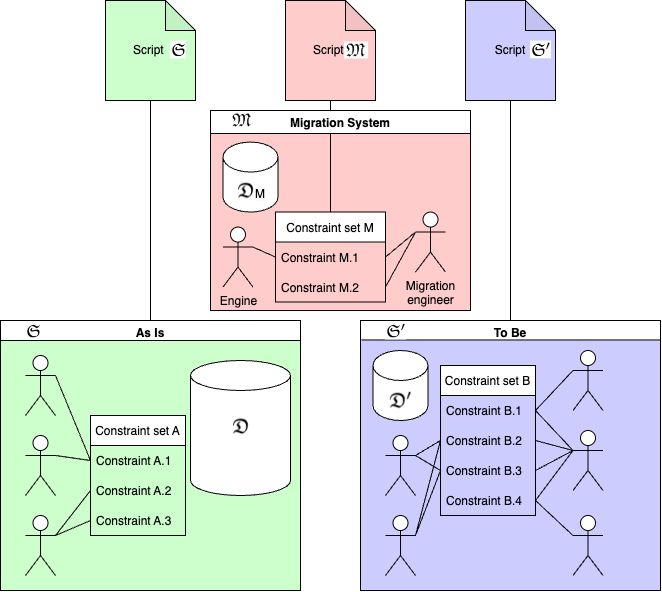
\includegraphics[scale=.45]{Migration.png}
   \end{center}
\caption{Data migration}
\label{fig:event flow}
\end{figure}
      
   We use two datasets: $\dataset$ and $\dataset'$.
   Before doing so, let us first define the disjoint union of two systems.
\begin{definition}[disjoint union of datasets]
\begin{eqnarray}
   \omit\rlap{$\la\atoms,\concepts,\inst,\isa,\rels,\dataset\ra\sqcup\la\atoms',\concepts',\inst',\isa',\rels',\dataset'\ra$}\notag\\
   &=&\la\atoms\uplus\atoms',\ \concepts\uplus\concepts',\ \inst\uplus^2\inst',\ \isa\uplus^2\isa',\ \rels\uplus^3\rels',\ \dataset\uplus^5\dataset'\ra\notag\\
      X\uplus Y&=&\{(x,0)\mid\ x\in X\}\ \cup\ \{(y,1)\mid\ y\in Y\}\\
      X\uplus^2 Y&=&\begin{array}[t]{@{}l}\{((x_1,0),(x_2,0))\mid\ (x_1,x_2)\in X\}\ \cup\\ \{((y_1,1),(y_2,1))\mid\ (y_1,y_2)\in Y\}\end{array}\\
      X\uplus^3 Y&=&\begin{array}[t]{@{}l}\{\declare{(n,0)}{(A,0)}{(B,0)}\mid\ \declare{n}{A}{B}\in X\}\ \cup\\ \{\declare{(n,1)}{(A,1)}{(B,1)}\mid\ \declare{n}{A}{B}\in Y\}\end{array}\\
      X\uplus^5 Y&=&\begin{array}[t]{@{}l}\{\triple{(a,0)}{\declare{(n,0)}{(A,0)}{(B,0)}}{(b,0)}\mid\ \triple{a}{\declare{n}{A}{B}}{b}\in X\}\ \cup\\ \{\triple{(a,1)}{\declare{(n,1)}{(A,1)}{(B,1)}}{(b,1)}\mid\ \triple{a}{\declare{n}{A}{B}}{b}\in Y\}\end{array}
\end{eqnarray}
\end{definition}
Note that if $\dataset$ and $\dataset'$ are datasets, then so is $\dataset\sqcup\dataset'$.

\subsection{Example}
   Let us proceed to specify a new system, $\infsys'$, to illustrate a (toy) migration.
   We will use the example in section~\ref{old IS} as the old system
   and call that $\infsys$ in this section.
   Its population reflects the state of the system just before the migration.

   Information system $\infsys'$, the new system, is specified by:
\begin{verbatim}
   RELATION takes[Student*Course]
   RELATION isPartOf[Module*Course] [UNI]=
      [ ("IT-Governance", "Business IT") ]
   RELATION isEnrolledFor [Student*Module] =
      [ ("Susan", "Business Analytics")
      ; ("Susan", "IT-Governance")
      ; ("Susan", "Business Rules")
      ]
   RULE EnrollRule: isEnrolledFor |- takes;isPartOf~
   ROLE Administrator MAINTAINS EnrollRule
   
   RELATION course[ExamReg*Course] [UNI] =
      [ ("ER1", "Management")
      ; ("ER2", "Business IT")
      ; ("ER3", "Business IT")
      ]
   RELATION student[ExamReg*Student] [UNI] =
      [ ("ER1", "Peter")
      ; ("ER2", "Susan")
      ]
   RULE ExamRule1: student~;course |- takes
   RULE ExamRule2: student~;course;isPartOf~ |- isEnrolledFor
\end{verbatim}
   This specification shows that $\infsys'$ gets to keep all three relations and the rule from $\infsys$.
   Some new population, two new relations, and two new rules have been added to $\infsys'$.
   $\infsys'$ contains exam registrations (concept \verb-ExamReg-), which is new.
   In an exam registration, a student registers for the examination of a course.
   $\infsys'$ contains two extra rules: \verb-ExamRule1- and \verb-ExamRule2-.
   The first one says that an exam registration requires that a student actually takes the course.
   In logic, the constraint $p_{\tt ExamRule1}$ is written as:
\[\begin{array}{l}\forall s\in\text{\tt Student}, e\in\text{\tt ExamReg}, c\in\text{\tt Course}:\\
   e\ \text{\tt student}\ s\ \wedge\ \ e\ \text{\tt course}\ c\ \rightarrow\ s\ \text{\tt takes}\ c\\
\end{array}\]
   Another requirement, \verb-ExamRule2-, is that the student is enrolled for every module that is part of the course.
   Its constraint, $p_{\tt ExamRule2}$, is written in logic as:
\[\begin{array}{l}\forall s\in\text{\tt Student}, e\in\text{\tt ExamReg}, m\in\text{\tt Module}, c\in\text{\tt Course}:\\
   e\ \text{\tt student}\ s\ \wedge\ \ e\ \text{\tt course}\ c\ \wedge\ m\ \text{\tt isPartOf}\ c\ \rightarrow\ s\ \text{\tt isEnrolledFor}\ m
\end{array}\]
   Ampersand also derives the following violation sets:
\[\begin{array}{l}
   \viol{\text{\tt ExamRule1}}{\dataset}\\
   \hspace{1cm}=\{\pair{s}{c}\mid\exists e:\ e\ \text{\tt student}\ s\ \wedge\ \ e\ \text{\tt course}\ c\ \wedge\neg(s\ \text{\tt takes}\ c)\}\\
   \viol{\text{\tt ExamRule2}}{\dataset}\\
   \hspace{1cm}=\{\pair{s}{m}\mid\exists e,c:\ e\ \text{\tt student}\ s\ \wedge\ \ e\ \text{\tt course}\ c\ \wedge\ m\ \text{\tt isPartOf}\ c\ \wedge\neg(s\ \text{\tt isEnrolledFor}\ m)\}
\end{array}\]

   So let us now turn to the migration.
   The intention of any migration is to preserve as much of the data from $\infsys$ as possible into $\infsys'$,
   while adding the new triples to $\infsys'$.
   So the first thing to do is to take the disjoint union of both systems.
   This yields:
\begin{verbatim}
   RELATION takes[Student*Course] =
      [ ("Peter", "Management")
      ; ("Susan", "Business IT")
      ; ("John", "Business IT")
      ]
   
   RELATION isPartOf[Module*Course] [UNI]=
      [ ("Finance", "Management")
      ; ("Business Rules", "Business IT")
      ; ("Business Analytics", "Business IT")
      ; ("IT-Governance", "Management")
      ; ("IT-Governance", "Business IT")
      ]
   
   RELATION isEnrolledFor [Student*Module] =
      [ ("Susan", "Business Analytics")
      ; ("Susan", "IT-Governance")
      ; ("Susan", "Business Rules")
      ]
   
   RULE EnrollRule: isEnrolledFor |- takes;isPartOf~
   ROLE Administrator MAINTAINS EnrollRule
   
   RELATION course[ExamReg*Course] [UNI] =
      [ ("ER1", "Management")
      ; ("ER2", "Business IT")
      ; ("ER3", "Business IT")
      ]
   RELATION student[ExamReg*Student] [UNI] =
      [ ("ER1", "Peter")
      ; ("ER2", "Susan")
      ]
   RULE ExamRule1: student~;course |- takes
   RULE ExamRule2: student~;course;isPartOf~ |- isEnrolledFor
\end{verbatim}
   If we check this for violations, we get the following results:
\begin{verbatim}
   There are 2 violations of RULE "ExamRule2":
      ("Peter", "IT-Governance")
      ("Peter", "Finance")
   ==============================
   There is one violation of RULE "UNI isPartOf[Module*Course]":
      ("IT-Governance", "IT-Governance")
\end{verbatim}
   Any data migration must anticipate any population in the old system.
   The only thing we know for sure about the ``old'' population is that it satisfies the rules in $\infsys$.

\subsubsection{Strategies for dealing with violations}

The violations of ExamRule2 don't pose a problem: they have a role (administrator) assigned to them.
We allow these violations to occur in the transition to the new system, and expect people with the Administrator role to deal with them.

However, the violations that arise when taking the (non-disjoint) union of the two scripts include violations of rules that the system should maintain.
This means that if we cannot generate software based on the disjoint union as it is.
To resolve this, the simplest solution is to change the roles assigned to the rules that are violated in the disjoint union:
\begin{verbatim}
   RELATION isPartOf[Module*Course]
   RULE isPartOfUNI: isPartOf;isPartOf~ |- I
   ROLE migrationHelper MAINTAINS isPartOfUNI
\end{verbatim}

Naturally, this solution requires effort from people with the role migrationHelper.
This in itself is not an issue: problems need to be solved one way or another.
However, a problem that may occur is that regular users of the system, who are used to the old system, might be adding data to the system that causes violations faster than they can be solved.
To mitigate this, we propose two solutions.

One solution is to state that the only violations that may occur in \verb=isPartOfUNI= are those that were present when the migration started:
\begin{verbatim}
   RELATION isPartOf[Module*Course]
   RULE isPartOfUNI: isPartOf;isPartOf~ |- I
   ROLE migrationHelper MAINTAINS isPartOfUNI
   
   RELATION isPartOfUNI_violations[Module*Module]
     = [("IT-Governance", "IT-Governance")]
   RULE isPartOfUNI_progress: -(isPartOf;isPartOf~) /\ I |- isPartOfUNI_violations
   SYSTEM MAINTAINS isPartOfUNI_progress
   
   ENFORCE isPartOfUNI_violations :< -(isPartOf;isPartOf~) /\ I  
\end{verbatim}

In this first solution, the first rule is the same as with the simple solution.
The second rule prevents any new violation from occurring.
Existing violations are recorded in the \verb=isPartOfUNI_violations= relation, and the rule \verb=isPartOfUNI_progress= prevents the set of violations to \verb=isPartOfUNI= from growing beyond this.
The \verb=ENFORCE= statement at the end of this code snippet states that the relation recording existing violations should be shrunk whenever violations are solved.
This way, we ensure that violations cannot re-occur.
As a whole, this means that \verb=migrationHelper= has a finite task.

As a second solution, we observe that the data in the designed system does not have any violations.
Consequentially, the cause of the violations comes from the triples in the old system.
Rather than taking the union of all triples, we can take the disjoint union instead;
\begin{verbatim}
   RELATION isPartOf_old[Module*Course] [UNI]=
      [ ("Finance", "Management")
      ; ("Business Rules", "Business IT")
      ; ("Business Analytics", "Business IT")
      ; ("IT-Governance", "Management")
      ]
   RELATION isPartOf[Module*Course] [UNI]=
      [ ("IT-Governance", "Business IT") ]
   RELATION isPartOf_ignored[Module*Course]
   
   RULE isPartOf_isUnion:  isPartOf_old :- isPartOf \/ isPartOf_ignored
   ROLE migrationHelper MAINTAINS isPartOf_isUnion
   
   ENFORCE isPartOf_ignored :> isPartOf
\end{verbatim}

\begin{verbatim}
   RELATION isPartOf_old[Module*Course] [UNI]=
      [ ("Finance", "Management")
      ; ("Business Rules", "Business IT")
      ; ("Business Analytics", "Business IT")
      ; ("IT-Governance", "Management")
      ]
   RELATION isPartOf[Module*Course] [UNI]=
      [ ("IT-Governance", "Business IT") ]
   RELATION isPartOf_ignored[Module*Course]

   ENFORCE isPartOf :> isPartOf_old - isPartOf_ignored
   ENFORCE isPartOf_ignored :> isPartOf
\end{verbatim}
In this second solution, we immediately move to a system in which the \verb=UNI= rule is maintained by the system.
The work for the \verb=migrationHelper= is again finite: the tuples in \verb=isPartOf_old= need to be copied over or explicitly ignored.
Once a tuple is in \verb=isPartOf=, the tuple is copied over to \verb=isPartOf_ignored= by the \verb=ENFORCE= statement, such that regular users can delete it without adding work to anyone with the \verb=migrationHelper= role.
Of course, since this solution starts with fewer pairs in the \verb=isPartOf= relation, other rules could be violated as a result of choosing this solution.
Indeed, ExamRule2 initially has more violations in this scenario.

\begin{definition}[migration dataset]
   \begin{eqnarray}
      &&\begin{array}[t]{@{}l}
         \{ {\tt ENFORCE\ }\declare{(nm',1)}{(A',1)}{(B',1)}\\\quad{\tt\ :=\ }\ident{(A',1)};\declare{(nm,0)}{(A,0)}{(B,0)};\ident{(B',1)}\\
            \mid\ \begin{array}[t]{@{}l}
               \declare{nm}{A}{B}\in\rels\wedge\declare{nm'}{A'}{B'}\in\rels'\wedge\id{nm}=\id{nm'}\ \wedge\\
               \{\pair{A}{A'},\pair{B}{B'}\}\subseteq\isa\cup\isa'\cup\flip{\isa}\cup\flip{\isa'}\}
               \end{array}
           \end{array}\\
           &\cup&\begin{array}[t]{@{}l}
            \{ {\tt CLASSIFY\ }(C',1){\tt\ IS\ }(C,0)\mid\ C\in\concepts,C'\in\concepts',C=C'\}\\
           \end{array}
   \end{eqnarray}
\end{definition}

The ${\tt CLASSIFY\ }(C',1){\tt\ IS\ }(C,0)$ statements add $((C',1),(C,0))$ and  $((C,0),(C',1))$ to the $\isa$ relation. Note that if $\dataset$ is a dataset, and $\dataset'$ is that dataset with pairs added\footnote{TODO: het woord `add' is informeel, dit kan beter} to the $\isa$ relation, then the result is again a dataset.
The ${\tt ENFORCE\ }r{\tt\ :=\ }e$ statements add triples $(x,r,y)$ for all $(x,y)\in e$.
The expressions $e$ in these statements are such that $x\ (\inst \compose \kleenestar{\flip{\isa}})\ (A',1)$ and $y \ (\inst \compose \kleenestar{\flip{\isa}})\ (B',1)$, thus preserving the property that the result is a dataset.

\begin{definition}[]
   \begin{eqnarray}
      \infsys\sqcup\infsys'&=&\la\roles',\rules',\maintain',\dataset\sqcup\dataset'\ra
   \end{eqnarray}
\end{definition}

\subsection{Changes}
% The purpose of this section is to explain why a dataset is structured the way it is.
   In the migration of a dataset we deal with changes to the elements that are not data:
   $\inst$, $\concepts$, and $\rels$.
   Such changes have further reaching consequences, however.
   Changes to $\inst$, $\concepts$, $\rels$ change the data structure in a dataset.
   We define a \define{migration of a dataset} $\la\atoms,\concepts,\inst,\rels,\dataset\ra$ as a change in which one or more of $\inst$, $\concepts$, or $\rels$ change.
   To satisfy the definition of datasets, $\dataset$ and $\atoms$ must change too,
   but the migration should try to preserve the maximal amount of data.

\section{Bibliography}
\bibliographystyle{elsarticle-harv}
\bibliography{doc}


\end{document}
